\documentclass[]{article}

%Packages
\usepackage{hyperref}
\usepackage[margin=1in]{geometry}
\usepackage{setspace}

\usepackage{graphicx}
\usepackage[usenames, dvipsnames]{color}
\usepackage{setspace}
\usepackage{float}

%Package Settings
\onehalfspacing
\setlength\parindent{0pt}


%opening
\title{DIME Dynamic Documentation Training \\ Stata Exercise}
\author{Luiza Andrade \& Mrijan Rimal}
\date{\today}

\makeatother

\begin{document}

\makeatletter
\begin{titlepage}
	\begin{center}
		
\includegraphics[width=0.3\linewidth]{i2i.png}\\[10ex]
		{\LARGE \bfseries  \@title }\\[2ex] 
		{\Large  \@author}\\[20ex] 
		{\large \@date}
	\end{center}
\end{titlepage}
\makeatother

\section*{Introduction}
This exercise introduces you to how to export files from Stata that can be read in {\LaTeX}. See exercise 1 and 2 for instructions on how to import file into {\LaTeX}. After this exercise and exercise 1, you will have a document that is automtically updated each time you run your Stata and your {\LaTeX} code.

We have provided you with a do-file that has code that creates file that you can import in a {\LaTeX} document. We will go through these examples and then we will ask you to create some tables and graphs of your own using your own data. Note that this is not an exercise on Stata, only on exporting in {\LaTeX} format from Stata, so this exercise assumes knowledge of some intermediate level Stata commands.

Start by opening the do-file \texttt{Export tables and images.do}, then move on with the exercise.


\section*{Setting your own path directories}

%Mrijan, add some text in the pragraph on organizing a folder neatly and to export to a single folder with descreptive names for it to not be too confusing when importing to LaTeX. For example, they should not export to the same folder where the do-file is. They should have an output folder with a fodler called raw, etc.

Exported tables and files should be in a folder that is accessible to {\LaTeX}. This means that extra care should be put in the first time you are typing out the path of the directory where the files are put. 


\textbf{Path} refers to location of the directory where the files are saved. \\

Before beginning the Stata exercises, we need to set our own paths to the global \texttt{main\_folder} and global \texttt{output} at the start of the do-file. This ensures that the graphs and figures are all saved in a directory {\LaTeX} can access. 

\subsection*{Finding Path on a Windows Computer}

Path to a file can be found by selecting a file and pressing {\color{red}SHIFT on your keyboard and RIGHT CLICKING your mouse and then clicking COPY AS PATH in the resulting drop down menu} as shown in Figure \ref{fig:pathwin3}.

\begin{figure}[H]
	\centering
	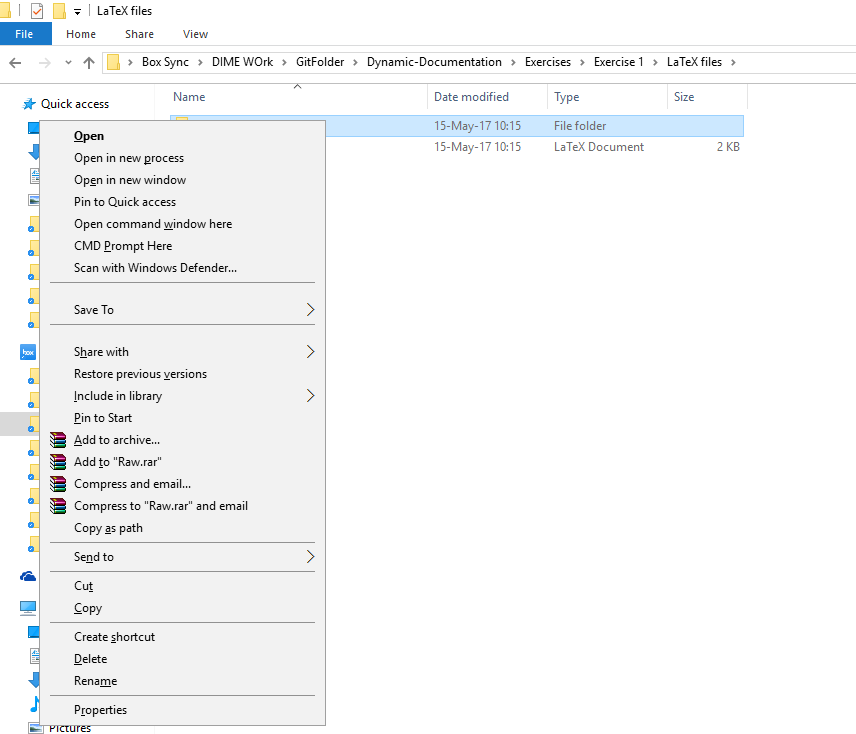
\includegraphics[width=0.9\linewidth]{pathwin3}
	\caption{Finding path on a Windows Computer - Solution 1}
	\label{fig:pathwin3}
\end{figure}

We can see in Figure \ref{fig:pathwin2}, that the complete path to the folder is show. We can then use this path when setting the path in our Stata do-file and change the path where it says \begin{verbatim}
global main_folder ``<<<ENTER YOUR FOLDER PATH HERE>>>''
\end{verbatim} 

Another solution to finding the path on a Windows computer is shown in Annex 1.
	
\subsection*{Finding Path on a Mac}


\section*{File formats}
The main things to consider while writing you do-file for dynamic documentation are as follows: 

The format that Stata exports should be readable by the {\LaTeX}. This means that when we export tables it will be exported in \texttt{.tex} format and when we export graphs it should be in \texttt{.png} format. 
The files will not be exported in \texttt{MS Word} or \texttt{MS Excel} format.

\section*{Task 1: Manually Create a Graph and then Export it}

This task shows us how to export graphs created in Stata to export in a format that {\LaTeX} can read. Using the \verb|graph export "$output/regular_graph.png", width(5000) replace| 
exports the graph in png format which {\LaTeX} can read. 
\section*{Exercise 2, Task 2: Using \texttt{iegraph} to create a figure}

This exercise teaches how to use \texttt{iegraph} to create a figure and export it to the graphs folder. \\

Using the \verb|save(``$output/iegraph.png'')| ensures that the graphs are directly saved to the \texttt{output} folder. 

\section*{Annex 1} {\label{annex1}}

\begin{figure}[H]
	\centering
	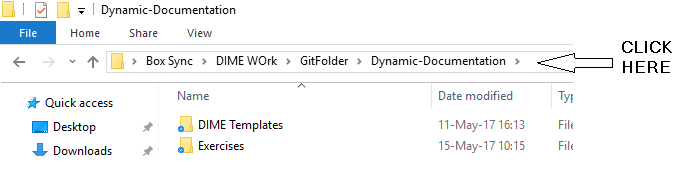
\includegraphics[width=1\linewidth]{pathwin}
	\caption{Finding Path on a Windows Computer}
	\label{fig:pathwin}
\end{figure}

As shown in Figure \ref{fig:pathwin}, left clicking(normal click) on the bar at the top of the \texttt{File Explorer} windows where our files are saved shows us the complete path to the files in a Windows computer. \\

\begin{figure}[H]
	\centering
	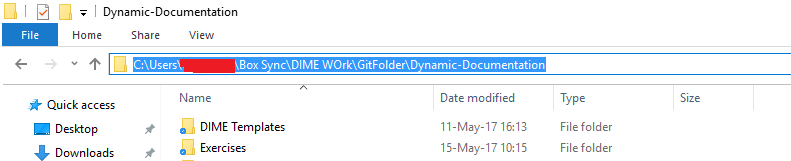
\includegraphics[width=1\linewidth]{pathwin2}
	\caption{Path shown on a Windows Computer}
	\label{fig:pathwin2}
\end{figure}

We can see in Figure \ref{fig:pathwin2}, that the complete path to the folder is show. We can then paste this path when setting the path in our Stata do-file and changing the path where it says \begin{verbatim}
global main_folder ``<<<ENTER YOUR FOLDER PATH HERE>>>''
\end{verbatim} 
	
\end{document}
